%%%%%%%%%%%%%%%%%%%%%%%%%%%%%%%%%%%%%%%%%%%%%%%%%%%%%%%
%                   File: OSAmeetings.tex             %
%                  Date: March 21, 2007  MSD          %
%                                                     %
%     For preparing LaTeX manuscripts for submission  %
%       submission to OSA meetings and conferences    %
%                                                     %
%       (c) 2007 Optical Society of America           %
%%%%%%%%%%%%%%%%%%%%%%%%%%%%%%%%%%%%%%%%%%%%%%%%%%%%%%%

\documentclass[letterpaper,10pt]{article}
\usepackage{osameet2}

%% standard packages and arguments should be modified as needed

\usepackage{amsmath,amssymb}

%\usepackage[pdftex,colorlinks=true,bookmarks=false,citecolor=blue,urlcolor=blue]{hyperref} %pdflatex
\usepackage[dvips,colorlinks=true,bookmarks=false,citecolor=blue,urlcolor=blue]{hyperref} %latex w/dvips

\begin{document}

\title{Understanding the Recovery Time of the Transceivers for High Speed Networks}

\author{Author name(s)}
\address{The Computer Laboratory, 15 , JJ Thomson Avenue, Cambridge, CB3 0FD}
\email{firstname.lastname@cl.cam.ac.uk}

\begin{abstract}
In this paper we present a simple testbed to measure the recovery time of the transceiver 
in a simple optical switch and provide some insights on how this can be reduced.
\end{abstract}

\ocis{000.0000, 999.9999.}


\section{Introduction}

One of the power hungry devices in the network components are the transceivers. In our previous
work \cite{yury}, we have described the power consumption of the various components in a transceiver and provided some insights on
how to address this. One approach is enforce the Lower Power Idle (LPI) state, which disables parts of phy 
(that are power hungry). The above approach lowers energy consumption but has a significant impact on the clock 
synchronization at the receiver due to the longer Phy recovery time (from the LPI state). This necessitates the 
requirement for faster clock recovery to avoid the dropping of packets.  In this paper we present a 
simple testbed to measure the recovery time of the transceiver in a simple optical switch and provide some 
insights on how the recovery time can be reduced.        


\section{Prototype}

This section gives an overview of the architecture of the complete system that was used to find 
the recovery time of the optical switch. The generator module inside the Virtex 5 FPGA of the NetFPGA-10G board \cite{blott}, generates traffic. Each packet that is generated has a sequence number (increases numerically)
and timestamp information embedded on it. This high speed traffic that is generated is sent to 
the MAC, where the XAUI uses transceivers to encode the data in 8b/10b coding and sends the 
traffic to the PHY chip (outside the FPGA). The PHY chip decodes the 8b/10b signal from the 
MAC, aligns it and encodes the traffic with 64b/66b encoding before sending it out of the board 
through the Ethernet ports. The Finisar SFP+ modules were connected to the Ethernet ports, 
which are terminated with LC connectors and multimode fibre is used. 

\begin{figure}[htbp]
  \centering
  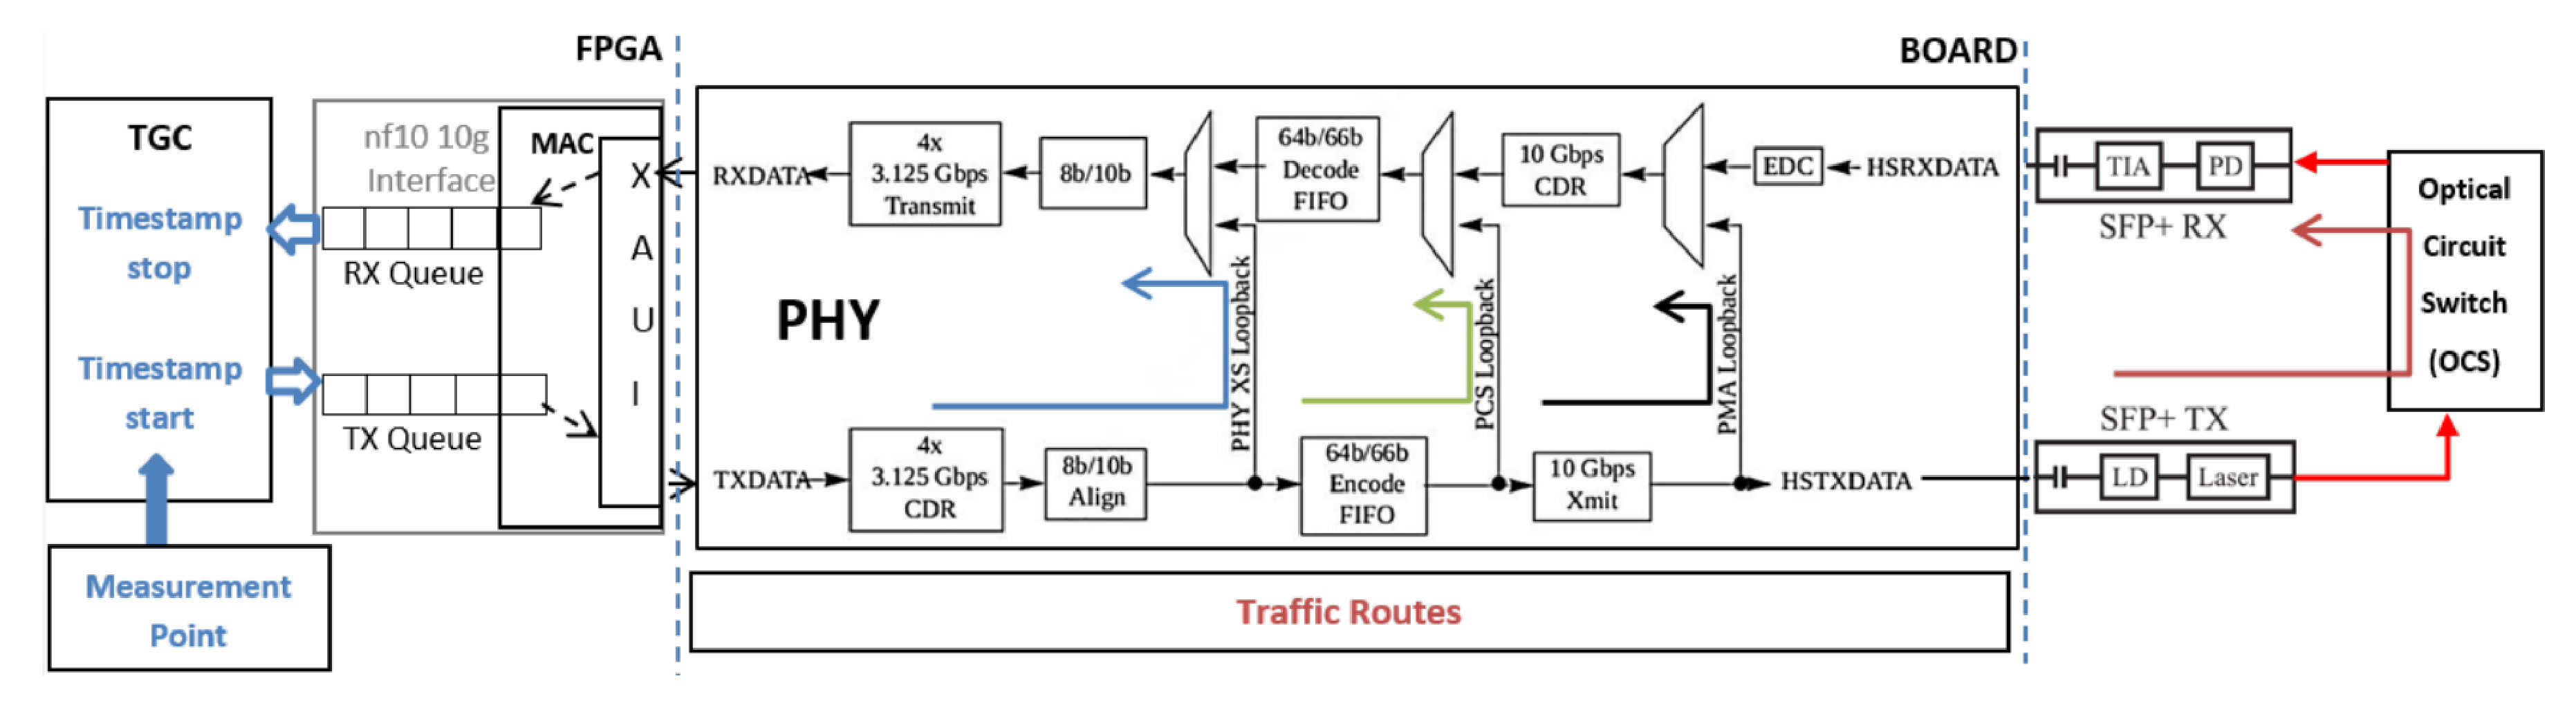
\includegraphics[width=15.3cm]{setup}
\caption{Prototype block diagram}
\end{figure}

The Switching element is a circuitry that drives the optical switch and is also controlled by 
the FPGA through the GPIO pins. A top level module inside the FPGA controls both the generator/checker 
module and the switch. The traffic that goes through the Switching element is, then, fed back into 
same port (for loopback measurements) or another port (for recovery time measurements) of the same board.

The receive path of the Phy does the complementary operation of the transmit path and passes the traffic to 
the checker module. The checker module puts a sequence number (numerically increasing) and 
timestamp information (using the same free running counter) on the packet and sends them to the host through
the PCIe interface. Using a user space application, packets are parsed to extract the round trip times.  


\section{Loopback measurements}



The Phy can be configured in three different loopback modes: PHY XS loopback, PCS loopback and PMA loopback. 
These loopback modes can be enabled or disabled by writing specific values to specific registers of the
AEL2005 device. The round trip time for the different loopback modes were obtained through our prototype explained
in the previous section. Need to update the results either as graph or table (TBD).

Authors in one observed that the total initialization time of the Feed Forward Equalizer (FFE) and the 
Distributed Feedback Equalizer (DFE) is about 600ms. They disabled the Electronic Dispersion Compensation (EDC) and
observed faster Clock and Data Recovery (CDR) initialization. 
  

\section{Recovery time measurements}

Will write some text and provide the diagram of the circuit, explaining which signals have been scoped. [TBD]
\begin{figure}[htbp]
  \centering
  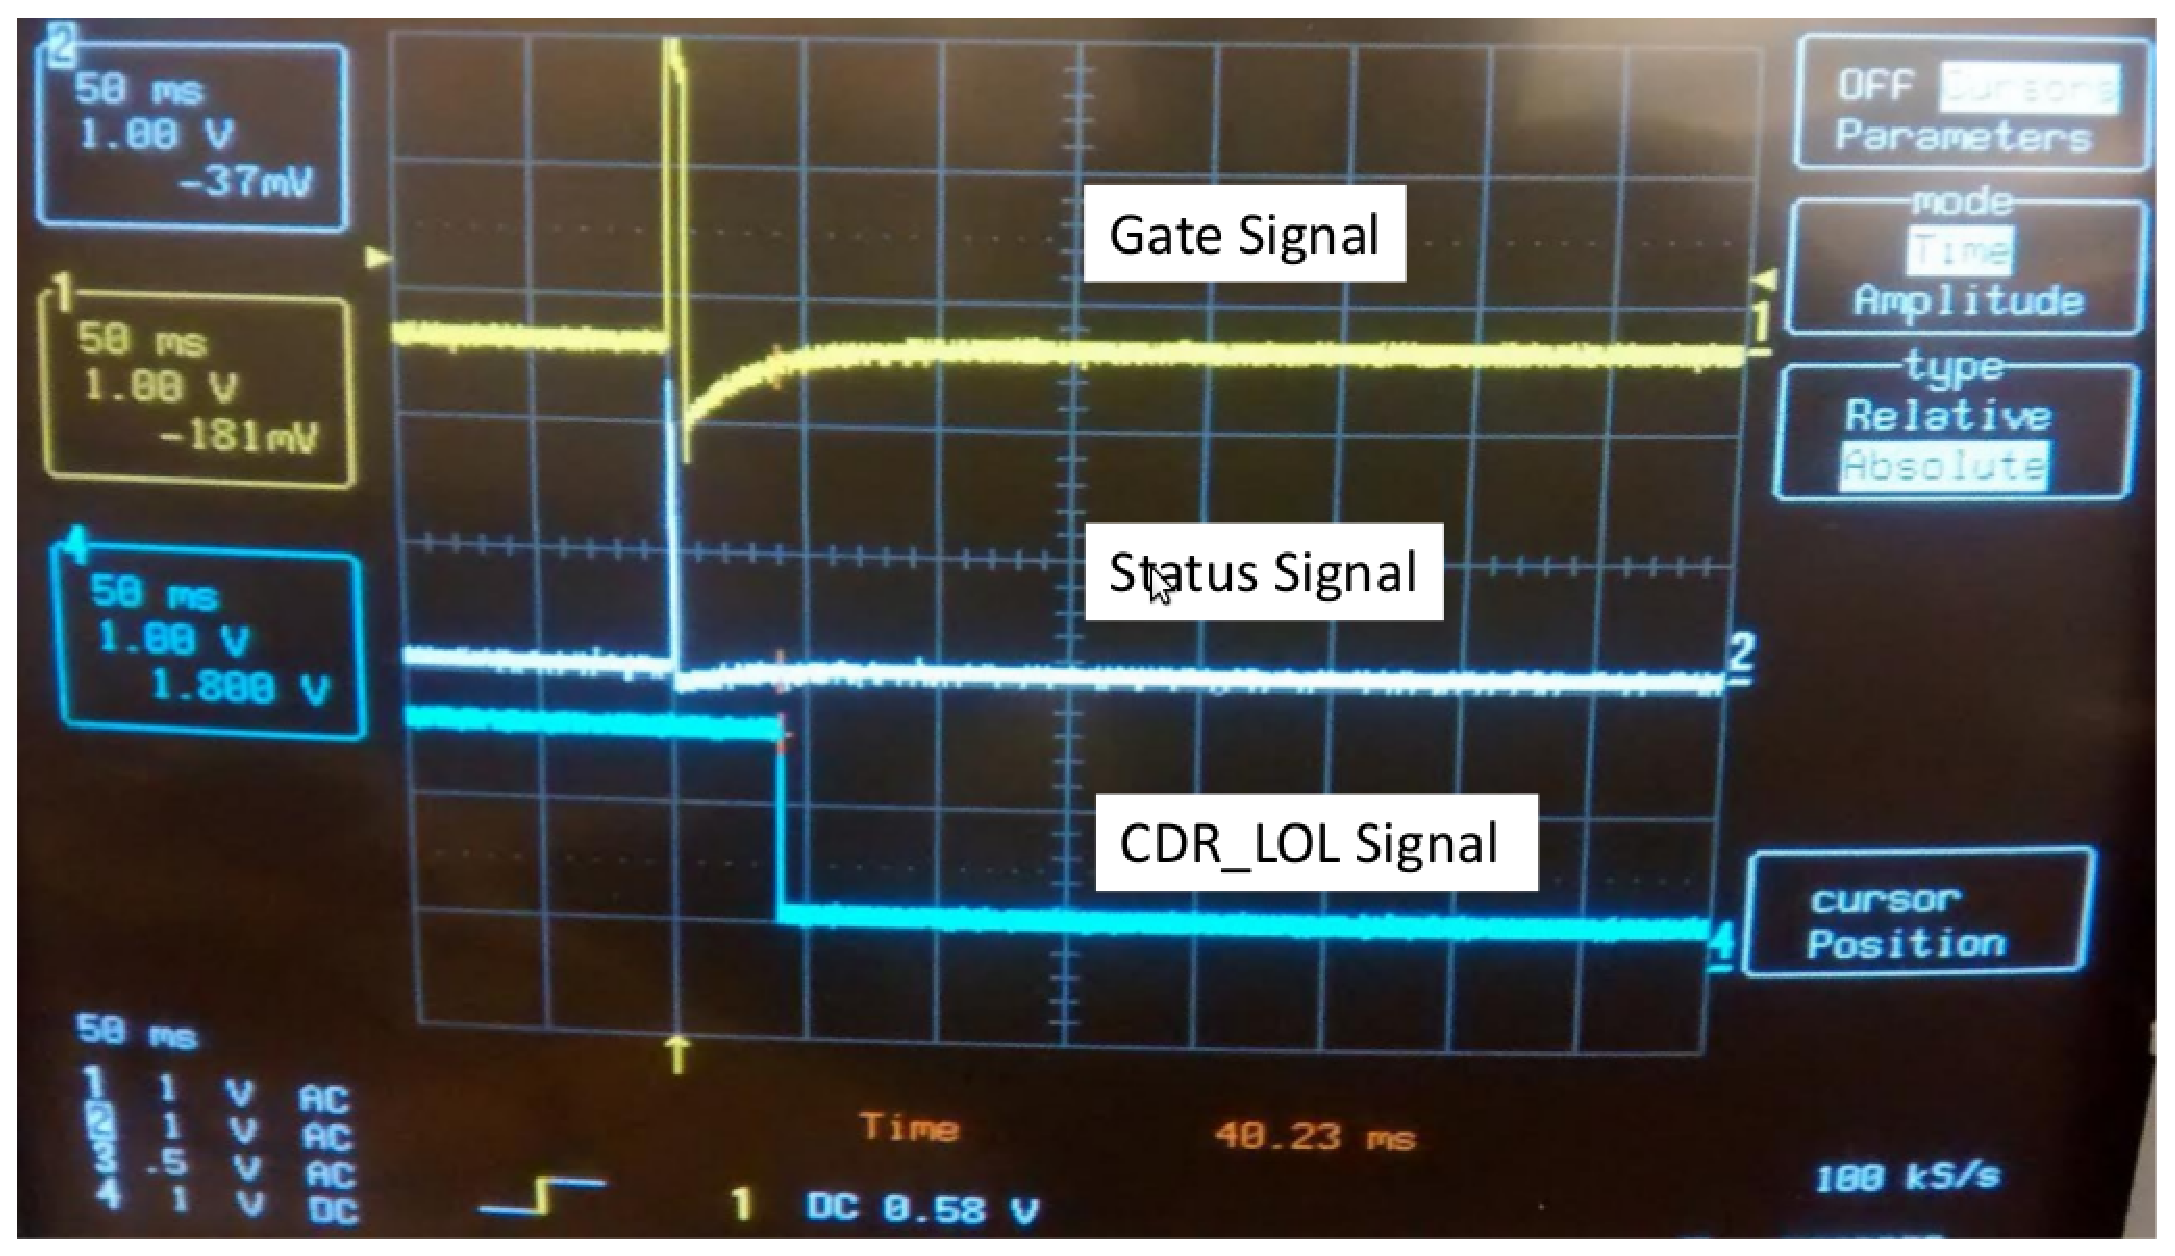
\includegraphics[width=15.3cm]{cdr}
\caption{Measurement of recovery time}
\end{figure}

\section{Reducing the recovery time}

Refer to M.Glick paper (TBD) and provide some insights.

\begin{thebibliography}{99}


\bibitem{helios} Farrington, Nathan, et al. "Helios: a hybrid electrical/optical switch architecture for modular data centers." ACM SIGCOMM Computer Communication Review 41.4 (2011): 339-350.

\bibitem{c-through} Wang, Guohui, et al. ``c-Through: Part-time optics in data centers.'' ACM SIGCOMM Computer Communication Review. Vol. 40. No. 4. ACM, 2010.

\bibitem{yury} Audzevich, Yury, et al. "Low power optical transceivers for switched interconnect networks." Advanced Technologies for Communications (ATC), 2013 International Conference on. IEEE, 2013. 

\bibitem{blott} Blott, Michaela, et al. ``FPGA research design platform fuels network advances.'' In Xilinx Xcell Journal, 73. 2010.
\end{thebibliography}


\end{document}
